\chapter{AM modulation and demodulation}
There're 3 types of AM modulation:
\begin{enumerate}
	\item DSBSC
	\item DSBFC
	\item SSBSC
\end{enumerate}

\section{Double Side Band Full carrier: DSBFC}
\setlength{\parindent}{0pt}

For message signal $m(t)$ and carrier $c(t)$, DSBFC is given by:
$$s(t) = (1 + k \times m(t)) c(t)$$

where $k$ is modulation order / modulation index


Demodulation can be done by a \underline{Square law demodulator}. Here modulated wave is squared and passed through a LPF (with cutoff near to message frequency). Additionally DC component can be removed (if needed).

\subsection*{Program}
\importMLCode{code/dsbfc.m}

\begin{figure}[H]
	\centering
	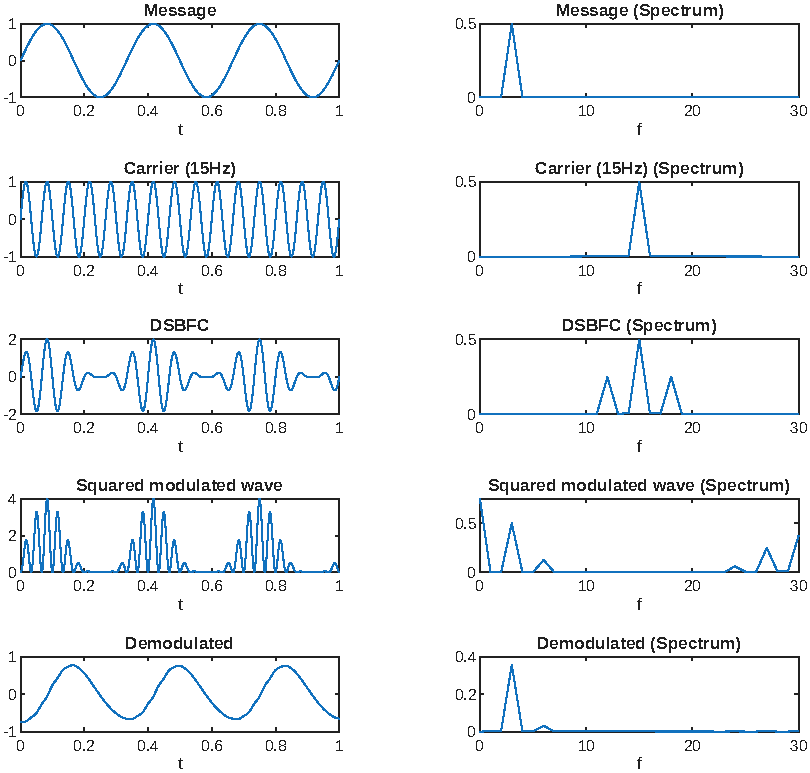
\includegraphics[width=\textwidth]{img/dsbfc.pdf}
\end{figure}

\pagebreak

\section{Double Side Band Suppressed carrier: DSBSC}

Modulation can be done using a \underline{balenced modulator}:

\begin{figure}[H]
	\centering
	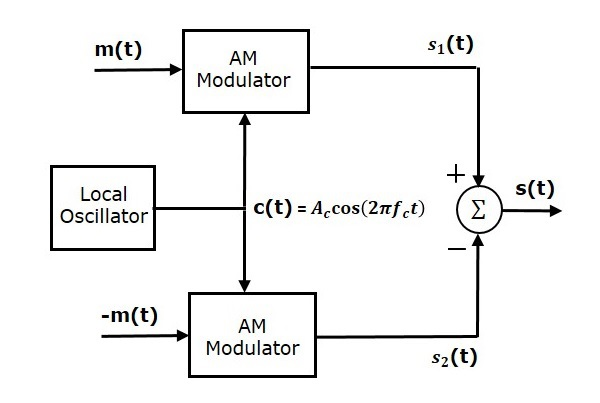
\includegraphics[width=.7\textwidth]{img/balanced_modulator.jpg}
\end{figure}
Hence expression for modulated wave is: 
\begin{align*}
	s(t) &= s_1(t) - s_2(t) \\
	 &= (1 + k \times m(t)) c(t) - (1 - k \times m(t)) c(t) \\
	 s(t)    &= 2k \times m(t) c(t)
\end{align*}

if we ignore $2k$ factor: 
$$s(t) = m(t)c(t)$$


Demodulation can be done by \underline{Coherent detection}: 
\begin{figure}[H]
	\centering
	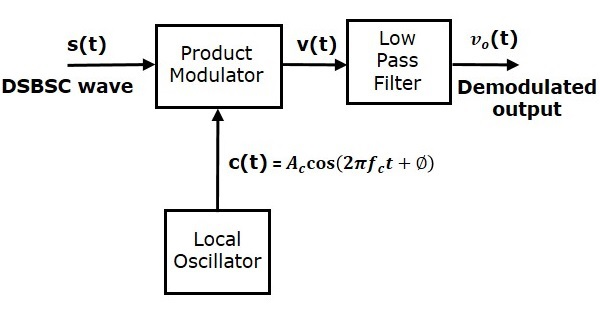
\includegraphics[width=.7\textwidth]{img/coh_detec.jpg}
\end{figure}

Hence demodulated output is: 
$$v_o(t) = \text{LPF}\left[s(t)\cdot c(t)\right]$$

\subsection*{Program}
\importMLCode{code/dsbsc.m}

\begin{figure}[H]
	\centering
	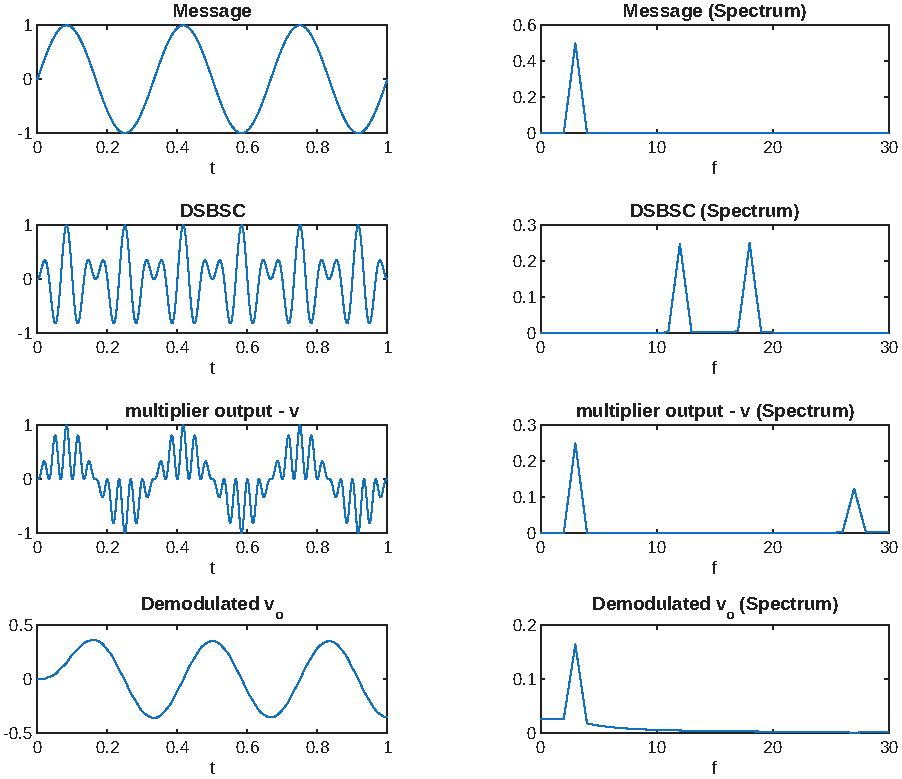
\includegraphics[width=\textwidth]{img/dsbsc.pdf}
\end{figure}

\section{Single Side Band Suppressed carrier: SSBSC}

A reliable Modulation method is  \underline{Frequency Discrimination Method}. This involves shifting phase of message and carrier signals. This can be done manually by writing their expressions, or by using using \href{https://en.wikipedia.org/wiki/Hilbert_transform}{Hilbert transform}.

\begin{figure}[H]
	\centering
	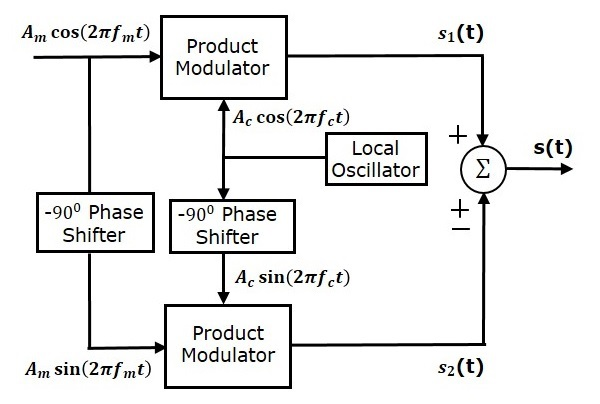
\includegraphics[width=.6\textwidth]{img/phase_disc.jpg}
\end{figure}
\subsection{Case where message and carrier are cos wave}
For a specific case of sine waves: 
if message is $m(t) = A_m \cos\left ( 2 \pi f_mt \right )$ and carrier is $c(t) = A_c \cos\left ( 2 \pi f_ct \right )$.

Product modulator output in top section is:
\begin{align*}
	s_1\left ( t \right )&=A_mA_c \cos \left ( 2 \pi f_mt \right ) \cos\left ( 2 \pi f_ct \right ) \\
	&=\frac{A_mA_c}{2} \left \{ \cos \left [ 2 \pi\left ( f_c+f_m \right )t \right ]+ \cos\left [ 2 \pi\left ( f_c-f_m \right )t \right ] \right \}
\end{align*}

In bottom section the message and the carrier signal are phase shifted by $-90^\circ$ before applying as inputs to the lower product modulator.

Therefore the output of lower product modulator is
\begin{align*}
	s_2\left ( t \right ) &=A_mA_c \cos\left ( 2 \pi f_mt-90^0 \right ) \cos\left (2 \pi f_ct-90^0  \right ) \\
	 &=\frac{A_mA_c}{2} \left \{ \cos \left [ 2 \pi\left ( f_c-f_m \right )t \right ]- \cos\left [ 2 \pi\left ( f_c+f_m \right )t \right ] \right \}
\end{align*}

To get lower sideband Add $s_1(t)$ and $s_2(t)$
\begin{align*}
	s(t) &= s_1(t) + s_2(t) \\
	\Aboxed{s(t)&=A_mA_c \cos \left [ 2 \pi\left ( f_c-f_m \right )t \right ]}
\end{align*}

To get upper sideband subtract $s_2(t)$ from $s_1(t)$
\begin{align*}
	s(t) &= s_1(t) - s_2(t) \\
	\Aboxed{s(t) &=A_mA_c \cos \left [ 2 \pi\left ( f_c+f_m \right )t \right ]}
\end{align*}

\subsection{General case (using Hilbert transform)}
Hilbert transform on a signal $x(t)$ provides $\pm 90^\circ$ phase shift to all frequencies present in the applied signal.
$-90^\circ$ phase shifted version of signal $x(t)$ can be obtained by taking imaginary part of Hilbert transform of the signal:
$$x'(t) = \mathfrak{Im}\{\mathcal{H}(x(t))\}$$

Hence the $s_2(t)$ can be written in terms of Hilbert transform as :
\begin{align*}
	s_2(t) &= \mathfrak{Im}\{\mathcal{H}(m(t))\}\times \mathfrak{Im}\{\mathcal{H}(c(t))\} \\
\end{align*}
From this lower side band can be obtained as:
$$s_{\text{LSB}}(t) = s_1(t) + s_2(t)$$
And upper side band can be obtained as:
$$s_{\text{USB}}(t) = s_1(t) - s_2(t)$$

\subsection{Demodulation}
Demodulation can be done by a coherent detector:
\begin{figure}[H]
	\centering
	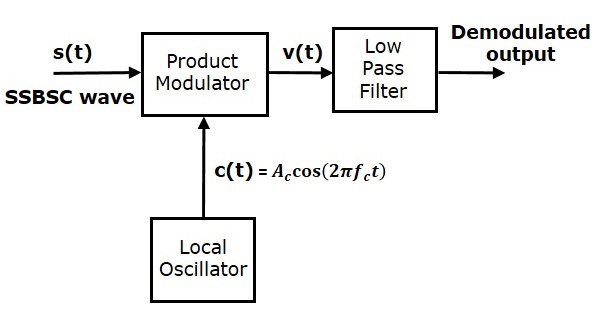
\includegraphics[width=.7\textwidth]{img/coh_detec2.jpg}
\end{figure}

\subsection*{Program (with Hilbert transform)}
Here I have demodulated the lower sideband. To get best result, cutoff frequency should be between $2f_m$ and $f_c$.

Message signal here is: $m(t) = 2\sin(2\pi f_m t^2);$
\importMLCode{code/ssbsc.m}

\begin{figure}[H]
	\centering
	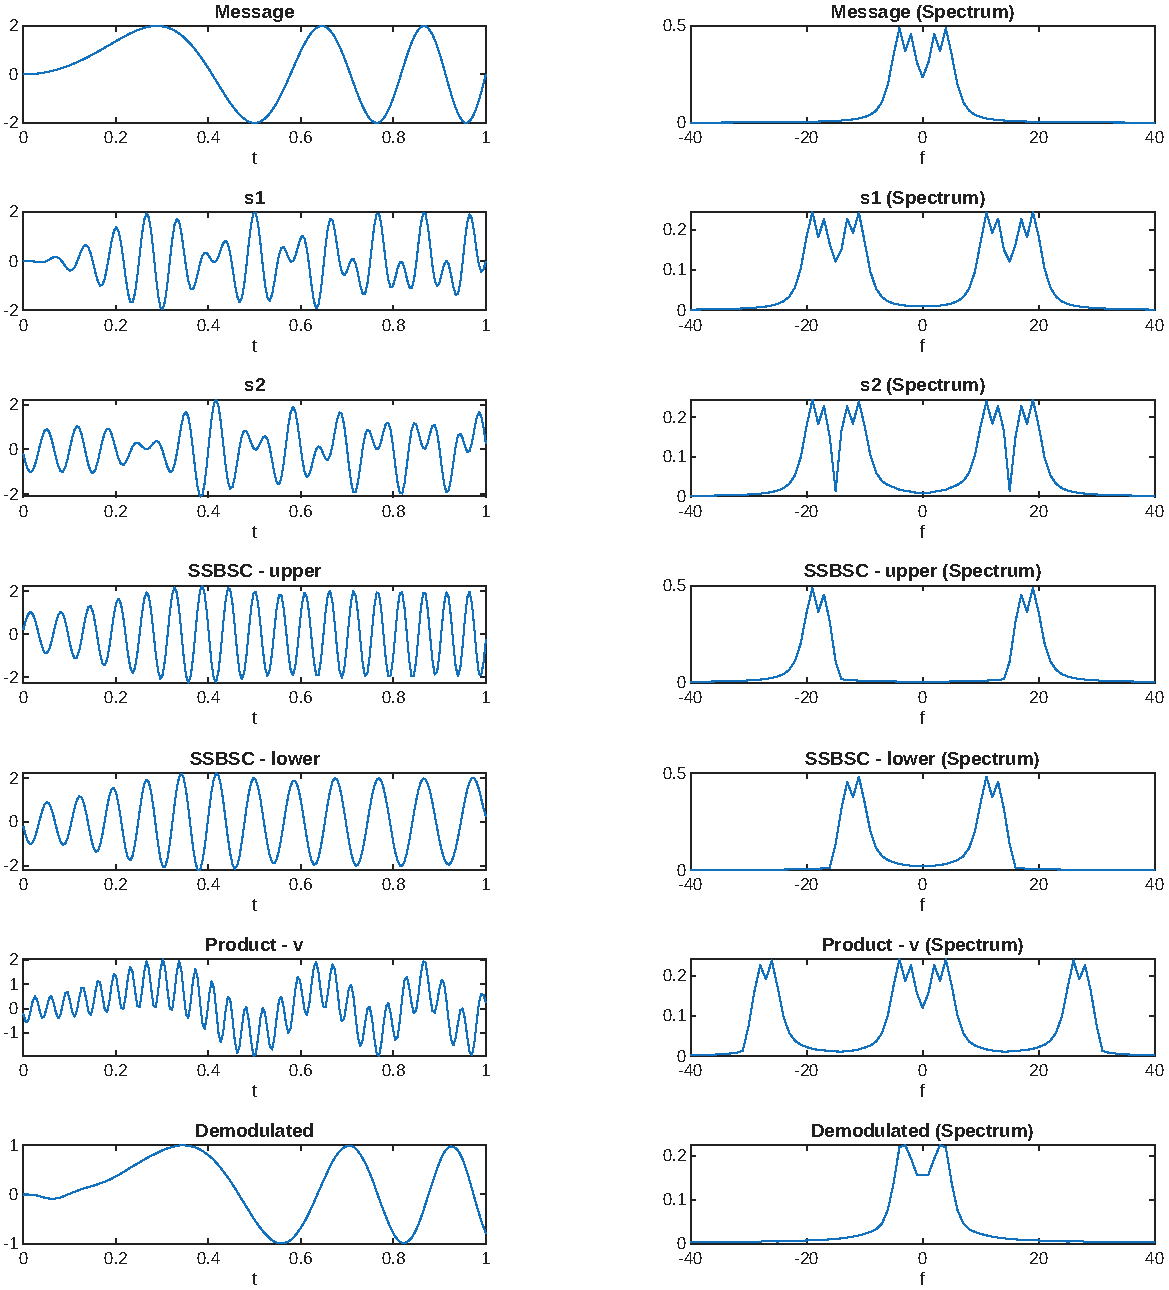
\includegraphics[width=\textwidth]{img/ssbsc.pdf}
\end{figure}

\pagebreak